\documentclass[12pt]{article}
\usepackage[brazil]{babel}
\usepackage{graphicx}
\usepackage{mathtools}
\usepackage{float} 
\usepackage{xcolor}


\usepackage{array}
\usepackage{booktabs}



% margenes
\usepackage[a4paper,left=2cm,right=2cm,top=1cm]{geometry}

%opening
\title{\textbf{Modelagem de Escoamentos Turbulentos. \\Lista de Exercícios No. 3}}

\author{Cristian Herledy López Lara}
\date{Junho 2025}

\begin{document}
	
\maketitle


\section*{Questão 1}

Obtenha a equação de transporte para o tensor de Reynolds\\


\textbf{\underline{Desenvolvimento}}

Partindo da equação de conservação de movimimento linear

\begin{equation}
	\frac{\partial U_i}{\partial t} + U_k \frac{\partial U_i}{\partial x_k} = \frac{1}{\rho} \frac{\partial P}{\partial x_i} + \nu \left( \frac{\partial ^ 2 U_i}{\partial x_k \partial x_k}\right) 
\end{equation}

Aplicando o conceito da media de Reynolds $A = \overline{A} + a$ para cada termo:

\begin{equation}
	\frac{\partial U_i}{\partial t} = \frac{\partial \overline{U_i} }{\partial t} + \frac{\partial u_i}{\partial t}
\end{equation}
\begin{equation}
	U_k \frac{\partial U_i}{\partial x_k} = \overline{U_k} \frac{\partial \overline{U_i}}{\partial x_k} + \overline{U_k} \frac{\partial u_i}{\partial x_k} + u_k \frac{\partial \overline{U_i}}{\partial x_k} + u_k \frac{\partial u_i}{\partial x_k} 
\end{equation}
\begin{equation}
	\frac{\partial P}{\partial x_i} = \frac{\partial \overline{P}}{\partial x_i} + \frac{\partial p}{\partial x_i}
\end{equation}
\begin{equation}
	\frac{\partial ^ 2 U_i}{\partial x_k \partial x_k} = \frac{\partial ^ 2 \overline{U_i}}{\partial x_k \partial x_k} +  \frac{\partial ^ 2 u_i}{\partial x_k \partial x_k}
\end{equation}

A equação completa fica então

\begin{equation}
	\frac{\partial \overline{U_i} }{\partial t} + \frac{\partial u_i}{\partial t} + \overline{U_k} \frac{\partial \overline{U_i}}{\partial x_k} + \overline{U_k} \frac{\partial u_i}{\partial x_k} + u_k \frac{\partial \overline{U_i}}{\partial x_k} + u_k \frac{\partial u_i}{\partial x_k} = \frac{1}{\rho} \frac{\partial \overline{P}}{\partial x_i} + \frac{\partial p}{\partial x_i} +  \frac{\partial ^ 2 \overline{U_i}}{\partial x_k \partial x_k} +  \frac{\partial ^ 2 u_i}{\partial x_k \partial x_k}
\end{equation}

Agora tomando só os termos da fluctuação turbulenta

\begin{equation}
	 \frac{\partial u_i}{\partial t} +  \overline{U_k} \frac{\partial u_i}{\partial x_k} + u_k \frac{\partial \overline{U_i}}{\partial x_k} + u_k \frac{\partial u_i}{\partial x_k} = \frac{1}{\rho} \frac{\partial p}{\partial x_i} +  \frac{\partial ^ 2 u_i}{\partial x_k \partial x_k}
\end{equation}

Multiplicando por $u_j$ cada termo da equação

\begin{equation}
	u_j\frac{\partial u_i}{\partial t} = \frac{\partial u_i u_j}{\partial t} - u_i \frac{\partial u_j}{\partial t}
\end{equation}

\begin{equation}
	u_j\overline{U_k} \frac{\partial u_i}{\partial x_k} = \overline{U_k} \frac{\partial u_i u_j}{\partial x_k} - \overline{U_k} u_i \frac{\partial u_i}{\partial x_k}
\end{equation}

\begin{equation}
	u_ju_k \frac{\partial \overline{U_i}}{\partial x_k} 
\end{equation}

\begin{equation}
	u_ju_k \frac{\partial u_i}{\partial x_k} = u_k \frac{\partial u_i u_j}{\partial x_k} - u_iu_k \frac{\partial u_j}{\partial x_k}
\end{equation}

\begin{equation}
	u_j\frac{\partial ^ 2 u_i}{\partial x_k \partial x_k} = \frac{\partial ^ 2 u_i u_j}{\partial x_k \partial x_k} - u_i\frac{\partial ^ 2 u_j}{\partial x_k \partial x_k}
\end{equation}

Escrevendo a equação completa:

\begin{equation}
	\begin{split}
		\frac{\partial u_i u_j}{\partial t} 
		- u_i \frac{\partial u_j}{\partial t} 
		+ \overline{U_k} \frac{\partial u_i u_j}{\partial x_k} 
		- \overline{U_k} u_i \frac{\partial u_i}{\partial x_k} 
		+ u_j u_k \frac{\partial \overline{U_i}}{\partial x_k} 
		+ u_k \frac{\partial u_i u_j}{\partial x_k} 
		- u_i u_k \frac{\partial u_j}{\partial x_k} 
		= \\
		\frac{u_j}{\rho} \frac{\partial p}{\partial x_i} +   \nu\left(  \frac{\partial ^ 2 u_i u_j}{\partial x_k \partial x_k} - u_i\frac{\partial ^ 2 u_j}{\partial x_k \partial x_k}\right) 
	\end{split}
\end{equation}

Da mesma forma, obtemos a equação para a flutuação $u_j$

\begin{equation}
	\begin{split}
		\frac{\partial u_i u_j}{\partial t} 
		- u_j \frac{\partial u_i}{\partial t} 
		+ \overline{U_k} \frac{\partial u_i u_j}{\partial x_k} 
		- \overline{U_k} u_j \frac{\partial u_j}{\partial x_k} 
		+ u_i u_k \frac{\partial \overline{U_i}}{\partial x_k} 
		+ u_k \frac{\partial u_i u_j}{\partial x_k} 
		- u_j u_k \frac{\partial u_j}{\partial x_k} 
		= \\
		\frac{u_i}{\rho} \frac{\partial p}{\partial x_i} + \nu \left(  \frac{\partial ^ 2 u_i u_j}{\partial x_k \partial x_k} - u_j\frac{\partial ^ 2 u_j}{\partial x_k \partial x_k}\right) 
	\end{split}
\end{equation}

Somando a equação 14 da equação 13 obtemos

\begin{equation}
	\begin{split}
		\frac{\partial u_i u_j}{\partial t} 		
		+ \overline{U_k} \frac{\partial u_i u_j}{\partial x_k} + u_j u_k \frac{\partial \overline{U_i}}{\partial x_k} + u_i u_k \frac{\partial \overline{U_i}}{\partial x_k} + \frac{\partial u_i u_j u_k}{\partial x_k}		
		= \\
		\frac{1}{\rho} \left( u_i\frac{\partial p}{\partial x_i} + u_j \frac{\partial p}{\partial x_j} \right) + \nu \left(  u_i\frac{\partial ^ 2  u_j}{\partial x_k \partial x_k} + u_j\frac{\partial ^ 2 u_i}{\partial x_k \partial x_k}\right) 
	\end{split}
\end{equation}

E aplicando os termos da media

\begin{equation}
	\begin{split}
		\frac{\partial \overline{u_i u_j}}{\partial t} 		
		+ \overline{U_k} \frac{\partial \overline{u_i u_j}}{\partial x_k} + \overline{u_j u_k} \frac{\partial \overline{U_i}}{\partial x_k} + \overline{u_i u_k} \frac{\partial \overline{U_i}}{\partial x_k} + \frac{\partial \overline{u_i u_j u_k}}{\partial x_k}		
		= \\
		\frac{1}{\rho} \left( \overline{u_i}\frac{\partial \overline{p}}{\partial x_i} + \overline{u_j} \frac{\partial \overline{p}}{\partial x_j} \right) + \nu \left(  \overline{u_i}\frac{\partial ^ 2  \overline{u_j}}{\partial x_k \partial x_k} + \overline
		{u_j}\frac{\partial ^ 2 \overline{u_i}}{\partial x_k \partial x_k}\right) 
	\end{split}
\end{equation}

\section*{Questão 2}

Simplifique a equação da energia cinética turbulenta $k = (u_i u_i)/2$ para o caso de um
escoamento médio turbulento plenamente desenvolvido em um duto.


\textbf{\underline{Desenvolvimento}}

Agora novamente da equação de transporte do tensor de Reynolds

\begin{equation}
	\begin{split}
		\frac{\partial \overline{u_i u_j}}{\partial t} 		
		+ \overline{U_k} \frac{\partial \overline{u_i u_j}}{\partial x_k} + \overline{u_j u_k} \frac{\partial \overline{U_i}}{\partial x_k} + \overline{u_i u_k} \frac{\partial \overline{U_i}}{\partial x_k} + \frac{\partial \overline{u_i u_j u_k}}{\partial x_k}		
		= \\
		\frac{1}{\rho} \left( \overline{u_i}\frac{\partial \overline{p}}{\partial x_i} + \overline{u_j}  \frac{\partial \overline{p}}{\partial x_j} \right) + \nu \left(  \overline{u_i}\frac{\partial ^ 2  \overline{u_j}}{\partial x_k \partial x_k} + \overline
		{u_j}\frac{\partial ^ 2 \overline{u_i}}{\partial x_k \partial x_k}\right) 
	\end{split}
\end{equation}

Façendo i=j e dividindo por 2 obtemos

\begin{equation}
	\begin{split}
		\frac{\partial k}{\partial t} 		
		+ \overline{U_k} \frac{\partial k}{\partial x_k} + k\frac{\partial \overline{U_i}}{\partial x_k} + k\frac{\partial \overline{U_i}}{\partial x_k} + u_k\frac{\partial k}{\partial x_k}		
		= \frac{1}{\rho} \left( \overline{u_i}\frac{\partial \overline{p}}{\partial x_i}  \right) + \nu \left(  \overline{u_i}\frac{\partial ^ 2  \overline{u_i}}{\partial x_k \partial x_k} \right) 
	\end{split}
\end{equation}

Para escoamento plenamente desenvolvido, a velocidade media na direçao i não muda com relaçao a j, então $\frac{\partial \overline{U_i}}{\partial x_k} = 0$

\begin{equation}
	\begin{split}
		\frac{\partial k}{\partial t} 		
		+ \overline{U_k} \frac{\partial k}{\partial x_k} + u_k\frac{\partial k}{\partial x_k}		
		= \frac{1}{\rho} \left( \overline{u_i}\frac{\partial \overline{p}}{\partial x_i}  \right) + \nu \left(  \overline{u_i}\frac{\partial ^ 2  \overline{u_i}}{\partial x_k \partial x_k} \right) 
	\end{split}
\end{equation}


\section*{Questão 3}
Demonstre (3.39) e mostre que (3.27) pode ser reescrita como 

\begin{equation}
	\overline{\varepsilon} = \nu \, \overline{ 
		\frac{\partial u_i}{\partial x_j} \frac{\partial u_i}{\partial x_j} } 
	+ \frac{\partial^2 \overline{u_i u_j}}{\partial x_i \partial x_j}
\end{equation}


\textbf{\underline{Desenvolvimento}}

A equação 3.39 é

\begin{equation}
	\frac{\overline{\partial u_i \partial u_j}}{\partial x_j \partial x_j} = \frac{\overline{\partial ^2 u_i u_j}}{\partial x_i \partial x_j}
\end{equation}

Abrindo o termo do lado dereito da equação 21

\begin{equation}
	\frac{\partial ^2 u_i u_j}{\partial x_i \partial x_j} = \frac{\partial}{\partial x_i} \left( \frac{\partial u_i u_j}{\partial x_j}\right) = \frac{\partial}{\partial x_i} \left ( u_i  \frac{\partial u_j}{\partial x_j} + u_j  \frac{\partial u_i}{\partial x_j} \right)
\end{equation}

Aplicando a igualdade da equação 3.6 $\frac{\partial u_i}{\partial x_i} = 0$

\begin{equation}
	\frac{\partial}{\partial x_i} \left (u_j  \frac{\partial u_i}{\partial x_j} \right) = \frac{\partial u_j }{\partial x_i}  \frac{\partial u_i}{\partial x_j} + u_j   \left ( \frac{\partial}{\partial x_i} \frac{\partial u_i}{\partial x_j} \right)
\end{equation}

Pela propiedade comutativa das derivadas parciais

\begin{equation}
	\frac{\partial u_j }{\partial x_i}  \frac{\partial u_i}{\partial x_j} + u_j   \left ( \frac{\partial}{\partial x_j} \frac{\partial u_i}{\partial x_i} \right) = \frac{\partial u_j }{\partial x_i}  \frac{\partial u_i}{\partial x_j}
\end{equation}

Agora igualando e aplicando as medias

\begin{equation}
	\frac{\overline{\partial u_i \partial u_j}}{\partial x_j \partial x_j} = \frac{\overline{\partial ^2 u_i u_j}}{\partial x_i \partial x_j}
\end{equation}


Agora para a equação 2.27 
\begin{equation}
	\overline{\varepsilon} = \frac{1}{2} \nu \, \overline{
		\left( \frac{\partial u_i}{\partial x_j} + \frac{\partial u_j}{\partial x_i} \right)
		\left( \frac{\partial u_i}{\partial x_j} + \frac{\partial u_j}{\partial x_i} \right)
	}
\end{equation}
Abrindo o producto dos termos

\begin{equation}
	\left( \frac{\partial u_i}{\partial x_j} + \frac{\partial u_j}{\partial x_i} \right)
	\left( \frac{\partial u_i}{\partial x_j} + \frac{\partial u_j}{\partial x_i} \right) = \frac{\partial u_i}{\partial x_j}\frac{\partial u_i}{\partial x_j} + \frac{\partial u_i}{\partial x_j}\frac{\partial u_j}{\partial x_i} + \frac{\partial u_j}{\partial x_i}\frac{\partial u_i}{\partial x_j} + \frac{\partial u_j}{\partial x_i}\frac{\partial u_j}{\partial x_i}
\end{equation}
 Agrupando os termos
 
\begin{equation}
	 \left( \frac{\partial u_i}{\partial x_j}\frac{\partial u_i}{\partial x_j} +  \frac{\partial u_j}{\partial x_i}\frac{\partial u_j}{\partial x_i} \right) + \left(  \frac{\partial u_i}{\partial x_j}\frac{\partial u_j}{\partial x_i} + \frac{\partial u_j}{\partial x_i}\frac{\partial u_i}{\partial x_j} \right) = 
	 \left( \frac{\partial u_i}{\partial x_j}\frac{\partial u_i}{\partial x_j} +  \frac{\partial u_i}{\partial x_j}\frac{\partial u_i}{\partial x_j} \right) + \left(  \frac{\partial u_i}{\partial x_j}\frac{\partial u_j}{\partial x_i} + \frac{\partial u_j}{\partial x_i}\frac{\partial u_i}{\partial x_j} \right)
\end{equation}

\begin{equation}
	2\left( \frac{\partial u_i}{\partial x_j}\frac{\partial u_i}{\partial x_j}  \right) + 2\left(  \frac{\partial u_i}{\partial x_j}\frac{\partial u_j}{\partial x_i} \right) = 2\left( \frac{\partial u_i}{\partial x_j}\frac{\partial u_i}{\partial x_j}  \right) + 2\left(  \frac{\partial ^2 u_i u_j}{\partial x_j \partial x_i} \right)
\end{equation}
Agora sustituindo em eq. 26

\begin{equation}
	\overline{\varepsilon} = \frac{1}{2} \nu \, \overline{2\left( \frac{\partial u_i}{\partial x_j}\frac{\partial u_i}{\partial x_j}  \right) + 2\left(  \frac{\partial ^2 u_i u_j}{\partial x_j \partial x_i} \right)} = \nu  \left[ \left( \overline{\frac{\partial u_i}{\partial x_j}\frac{\partial u_i}{\partial x_j}  }\right) + \left(  \frac{\partial ^2 \overline{u_i u_j}}{\partial x_j \partial x_i} \right)\right] 
\end{equation}

\section*{Questão 4}



Usando correlações para camada limite turbulenta sobre uma superfície plana disponíveis em livros texto da graduação, determine os valores de $U\infty/u^*$, $Re_\delta$ e Re* em x = 1 e 2 m.\\

\textbf{\underline{Desenvolvimento}}

A expressão para o comprimento da camada limite turbulenta é definida como

\begin{equation}
	\delta = 0,382 x Re_x^{-1/5}
\end{equation}


Calculando os valores para $x=1m$

\begin{equation}
	Re_x = \frac{U_\infty x}{\nu} = \frac{25 \frac{m}{s} \cdot 1m}{1,5 x 10 ^{-5} m^2 / s} = 1,66 x 10 ^ {6}
\end{equation}

\begin{equation}
	\delta_{1m}= 0,382 x Re_x^{-1/5} = 0,382 \cdot 1m \cdot(1,66 x 10 ^ {6})^{-1/5} = 0,021 m
\end{equation}

\begin{equation}
	Re_\delta = \frac{U_\infty \delta}{\nu} = \frac{25 \frac{m}{s} \cdot 0,021m}{1,5 x 10 ^{-5} m^2 / s} = 3.5 x 10 ^ 4
\end{equation}

Calculando os valores para $x=2m$

\begin{equation}
	Re_x = \frac{U_\infty x}{\nu} = \frac{25 \frac{m}{s} \cdot 2m}{1,5 x 10 ^{-5} m^2 / s} = 3,33 x 10 ^ {6}
\end{equation}

\begin{equation}
	\delta_{1m}= 0,382 x Re_x^{-1/5} = 0,382 \cdot 2m \cdot (3,33 x 10 ^ {6})^{-1/5} = 0,036 m
\end{equation}

\begin{equation}
	Re_\delta = \frac{U_\infty \delta}{\nu} = \frac{25 \frac{m}{s} \cdot 0,036m}{1,5 x 10 ^{-5} m^2 / s} = 6 x 10 ^ 4
\end{equation}

Considerando o modelamiento da velocidade dado pela expressão de la lei logarítmica (eq 3.210 de [1])

\begin{equation}
	\frac{U_\infty}{u_*} + \frac{1}{\kappa} \ln\left( \frac{U_\infty}{u_*} \right)
	= \frac{1}{\kappa} \ln Re_\delta + a - b
\end{equation}

Onde (de [1])

\begin{equation}
	Re_\delta = \dfrac{U_\infty}{u^*} Re_*
\end{equation}

Da eq. 38, encontra-se o valor de $u_*$ para $x=1m$, com os valores de $k\approx 0,41 ; a = 5,2 ; b = -2,5$

\begin{equation}
	\frac{25}{u_*} + \frac{1}{0,41} \ln\left( \frac{25}{u_*} \right)
	= 44,3\  \rightarrow \ u_*= 0,70 m/s
\end{equation}

\begin{equation}
	\frac{U_\infty}{u_*} = \frac{25 m/s}{0,70m/s} = 35,7
\end{equation}


E para $x = 2m$

\begin{equation}
	\frac{25}{u_*} + \frac{1}{0,41} \ln\left( \frac{25}{u_*} \right)
	= 35,5 \  \rightarrow \ u_*= 0,95 m/s
\end{equation}

\begin{equation}
	\frac{U_\infty}{u_*} = \frac{25 m/s}{0,95m/s} = 26,1
\end{equation}

\section*{Questão 5}

Considere o escoamento turbulento plenamente desenvolvido de água em uma tubulação
circular de parede lisa com raio R.\\
a) Assumindo que a espessura da subcamada limite viscosa $\delta_v$ é equivalente a y+ = 5, mostre
em um gráfico log-log, a razão $\delta_v/R$ para números de Reynolds $=( UD/\nu)$ iguais a $10^4$, $10^5$ e $10^6$. Use alguma correlação, como a de Blasius, para determinar a tensão na parede.\\
b) Represente em um gráfico a distribuição de velocidade $U(r)/U$ para cada um dos números de
Reynolds.\\
c) Avalie o valor local da velocidade média em y+ = 5 e 50.\\

\textbf{\underline{Desenvolvimento}}

a) O primer paso é emcontar uma expressão para $\delta_v$. Da definição da expesura da subcamada límite viscosa

\begin{equation}
	y^+ = 5 = \frac{u_*\delta_v}{\nu}
\end{equation}
\begin{equation}
	\delta_v = \frac{5\nu}{u_*} \ \rightarrow \ \frac{\delta_v}{R} = \frac{5\nu}{Ru_*}
\end{equation}

Da expressão da velocidade de atrito e do coeficiente de atrito $f$

\begin{equation}
	u_*=\sqrt{\frac{\tau_w}{\rho}} \ ; \ f = \frac{\tau_w}{\frac{1}{2}\rho U^2} \ \rightarrow \ u_*=\sqrt{\frac{f}{2}}U
\end{equation}
Da definição do número de Reynolds

\begin{equation}
	Re_D = \frac{UD}{\nu} \ \rightarrow \ U= \frac{Re \nu}{D}
\end{equation}

Sustituindo em (46)

\begin{equation}
	u_*=\sqrt{\frac{f}{2}}U \ \rightarrow \  u_*=\sqrt{\frac{f}{2}} \frac{Re \nu}{D}
\end{equation}

Agora, reescrevendo na equação (45)

\begin{equation}
	\frac{\delta_v}{R} = \frac{5\nu}{Ru_*} = \frac{5\nu}{R\sqrt{\frac{f}{2}} \frac{Re \nu}{D}}
\end{equation}

Façendo manipulações algebraicas obtem-se que

\begin{equation}
	\frac{\delta_v}{R} = \frac{10 \cdot 2^{1/2}}{Re f^{1/2}}
\end{equation}

Pela correlação de Blasius que relaciona o coeficiente de atrito com o número de Reynolds

\begin{equation}
	f = 0,316 Re^{-1/4}
\end{equation}

Agora sustituindo em (51)

\begin{equation}
	\frac{\delta_v}{R} = \frac{10 \cdot 2^{1/2}}{Re (0,316 Re^{-1/4})^{1/2}} = \frac{10 \cdot 2^{1/2}}{Re^{7/8} \cdot 0,316^{1/2}}
\end{equation}

Obtem-se então uma razão para $\delta_v/R$ em função de $Re$

\begin{equation}
	\frac{\delta_v}{R} = 25,1 Re^{-7/8}
\end{equation}

O seguinte gráfico mostra como essa relação evolui com 3 números de Reynolds diferentes

\begin{figure}[H]
	\centering
	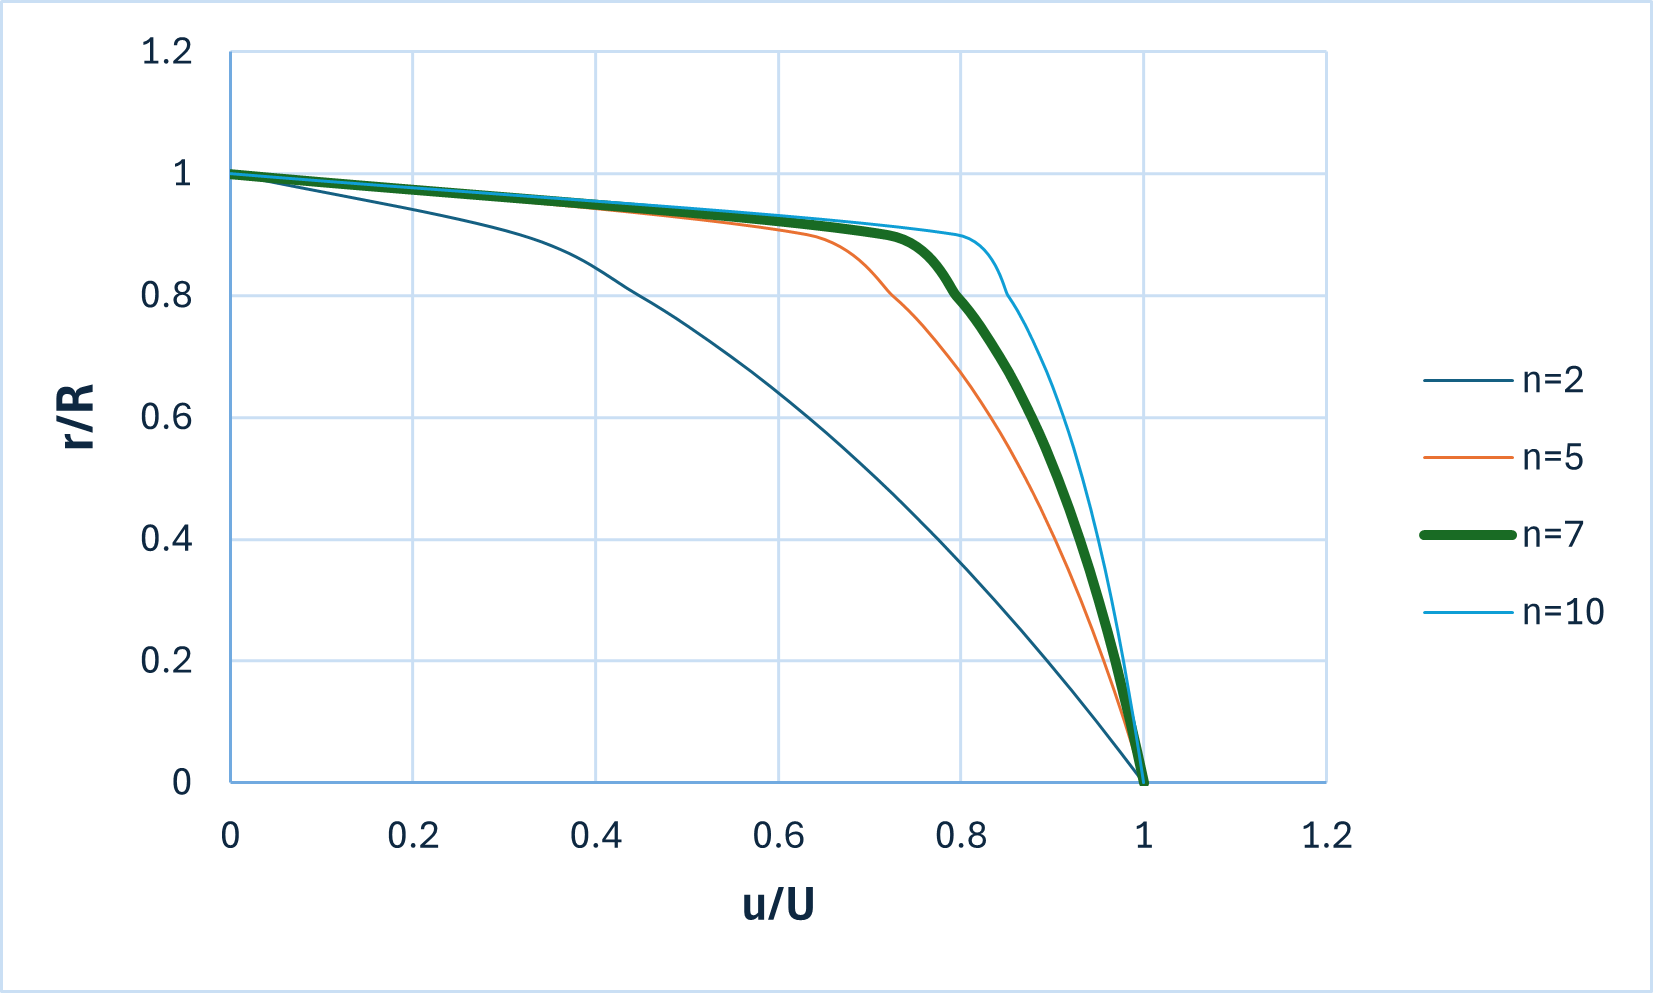
\includegraphics[width=.65\textwidth]{figures/1}
	\caption{Evalução da razão $\delta_v/R$ vs $Re$}
\end{figure}

O gráfico mostra como o tamanho da camada límite viscosa diminui a medida que a velocidade media va aumentando.\\

b) Para a distribução de velocidade, façemos uso da dependencia logaritmica do valor de $U(y)/u_*$ em Re

\begin{equation}
	\frac{U(y)}{u_*} = \frac{1}{\kappa} \ln\left( y^+ \right) + a
\end{equation}

Podemos aplicar a relação $y = R(1-\frac{r}{R})$ em a eq. (44)

\begin{equation}
	y^+  = \frac{u_*\delta_v}{\nu} \ = \ \frac{u_*R(1-\frac{r}{R})}{\nu}
\end{equation}

Sustituindo em (54)

\begin{equation}
	\frac{U(r)}{u_*} = \frac{1}{\kappa} \ln\left( \frac{u_*R(1-\frac{r}{R})}{\nu} \right) + a
\end{equation}

Agora, para emcontrar uma expressão que relacõe a velocidade radial $U(r)$ com a velocidade media $U$, podemos usar as expressões calculadas anteriormenete para $u_*$ que são as duas definições da equação (48), obtendo

\begin{equation}
	\frac{U(r)}{U} = \frac{0,39}{\kappa} Re^{1/8} \ln\left( \frac{Re^{7/8}(1-\frac{r}{R})}{2} \right) + a
\end{equation}

Então, o comportamento da distribução de velocidade em funcão de Reynolds, pode ser analisado no gráfico a seguir, onde $k = 0,41$ e $a=5.2$

\begin{figure}[H]
	\centering
	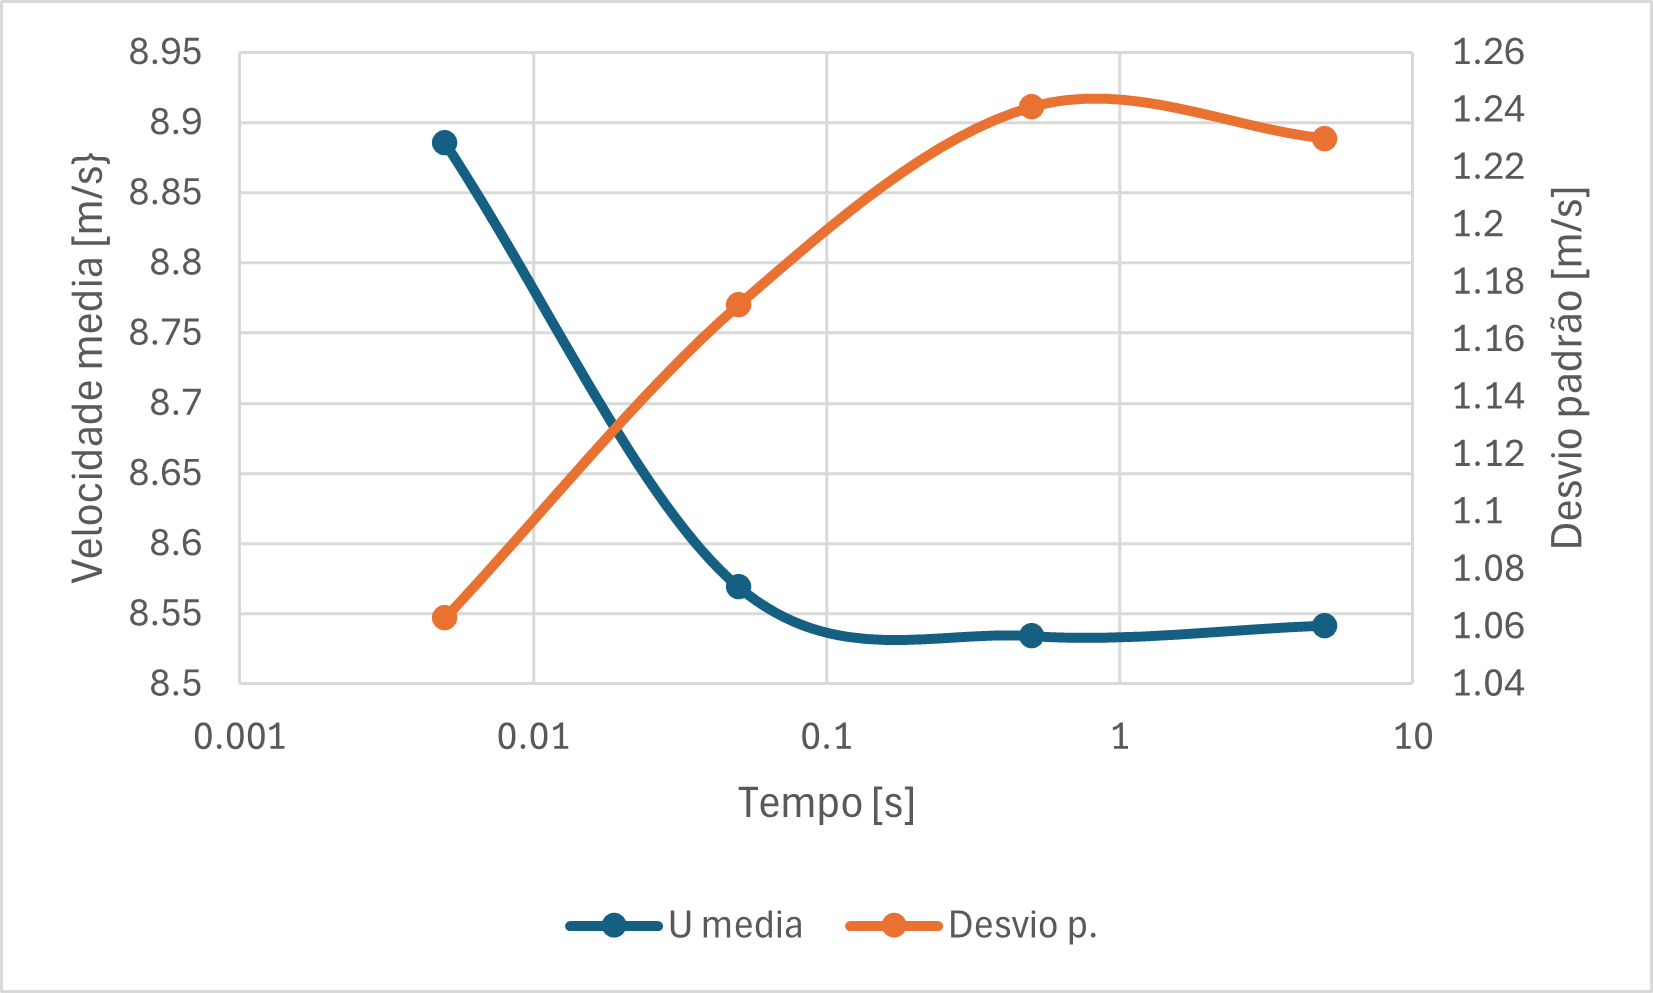
\includegraphics[width=.65\textwidth]{figures/2}
	\caption{Evalução da distribução de velocidade em funcão de Reynolds vs $Re$}
\end{figure}


À medida que o número de Reynolds aumenta, o perfil de velocidade torna-se mais plano no centro e com um gradiente maior na parede. Isso reflete o fortalecimento dos efeitos inerciais e turbulentos e a formação de uma camada limite fina que governa a dissipação de energia e a tensão de cisalhamento.

c) Para a avaliação da velocidade media, novamente da equãcao (57) obtemos que 

\begin{equation}
	\frac{U(r)}{U} = \frac{1}{\kappa} \ln\left( y^+ \right) + a = \frac{1}{\kappa} \ln\left( \frac{u_*R(1-\frac{r}{R})}{\nu} \right) + a
\end{equation}

Os seguintes valores da distribuçao de velocidade foram obtidos

\begin{table}[H]
	\centering
	\begin{tabular}{|c|c|c|}
		\hline
		Re  & y+ & U(y)/U \\ \hline
		$10^4$   & 5   & 10,0   \\ \hline
		$10^4$   & 50   & 17 \\ \hline
		$10^5$   & 5    & 11,6    \\ \hline
		$10^5$    & 50   & 20,8  \\ \hline
		$10^6$   & 5    & 13,8    \\ \hline
		$10^6$    & 50   & 26   \\ \hline
	\end{tabular}
	\caption{Valores de velocidade obtidos com Re y $y^+$}
\end{table} 

Os valores obtidos mostram que, para posições diferentes da parede ($y^+ = 5 \ e \ 50$), a velocidade  cresce com o aumento do número de Reynolds. Além disso, o gradiente de velocidade também cresce com $Re$, indicando que a região de cisalhamento se torna mais fina e intensa, característica típica de escoamentos turbulentos com alto Reynolds.

\section*{Questão 6}
A partir da proposta de Coles para uma camada limite turbulenta, represente o perfil de
velocidade para uma camada limite com gradiente de pressão nulo, favorável (b = 10) e adverso (b = - 10). Represente o perfil de velocidade para a condição de separação ($b\rightarrow\infty$).\\


\textbf{\underline{Desenvolvimento}}\\
Da expressão proposta por Coles para a lei do déficit de velocidade na região externa

\begin{equation}
	F(\eta) = \frac{1}{k} ln(\eta) + b\left[ 1-\frac{w(\eta)}{2}\right] 
\end{equation}

Onde a função universal é dada por


\begin{equation}
	w(\eta)= 1 - cos(\pi\eta) 
\end{equation}

Variando o parámetro b, variacões devido ao gradiente pressão serám observadas.

\begin{figure}[H]
	\centering
	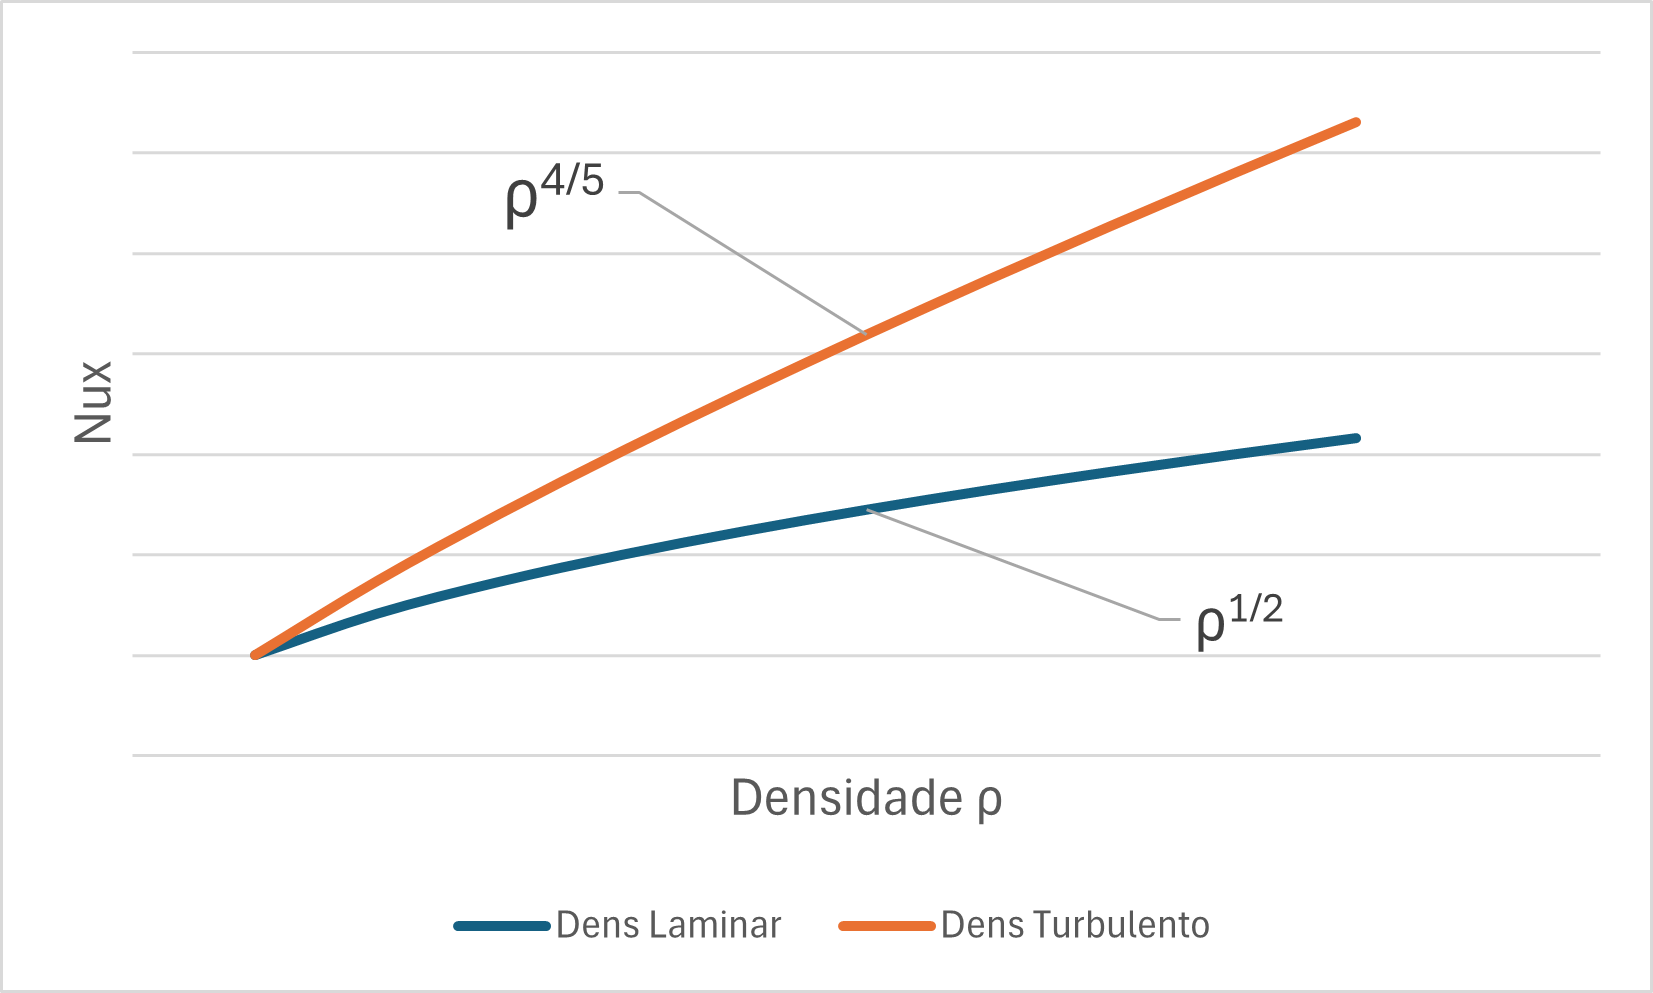
\includegraphics[width=.65\textwidth]{figures/3}
	\caption{Déficit de velocidade para diferentes niveis de gradiente de pressão}
\end{figure}

A figura mostra o déficit de velocidade na camada externa, observando-se como muda a região de trabalho da lei logarítmica com as variacões do gradiente de pressão (favorável = 10, adverso = -10 e nulo =-2). Para o gradiente adverso, um aumento da espesura da camada límite é observada pelo alto nivel do déficit. Mas, para o gradiente favorável tem uma disminução da camada limite pela acelerção do escoamento.




Dado que 
\begin{equation}
	F(\eta) = \frac{U_\infty - U}{u_*}
\end{equation}

O perfil de velocidade adimensional $U/U_\infty$ pode ser analisado em função de $\eta$ como é mostrado no seguinte gráfico

\begin{figure}[H]
	\centering
	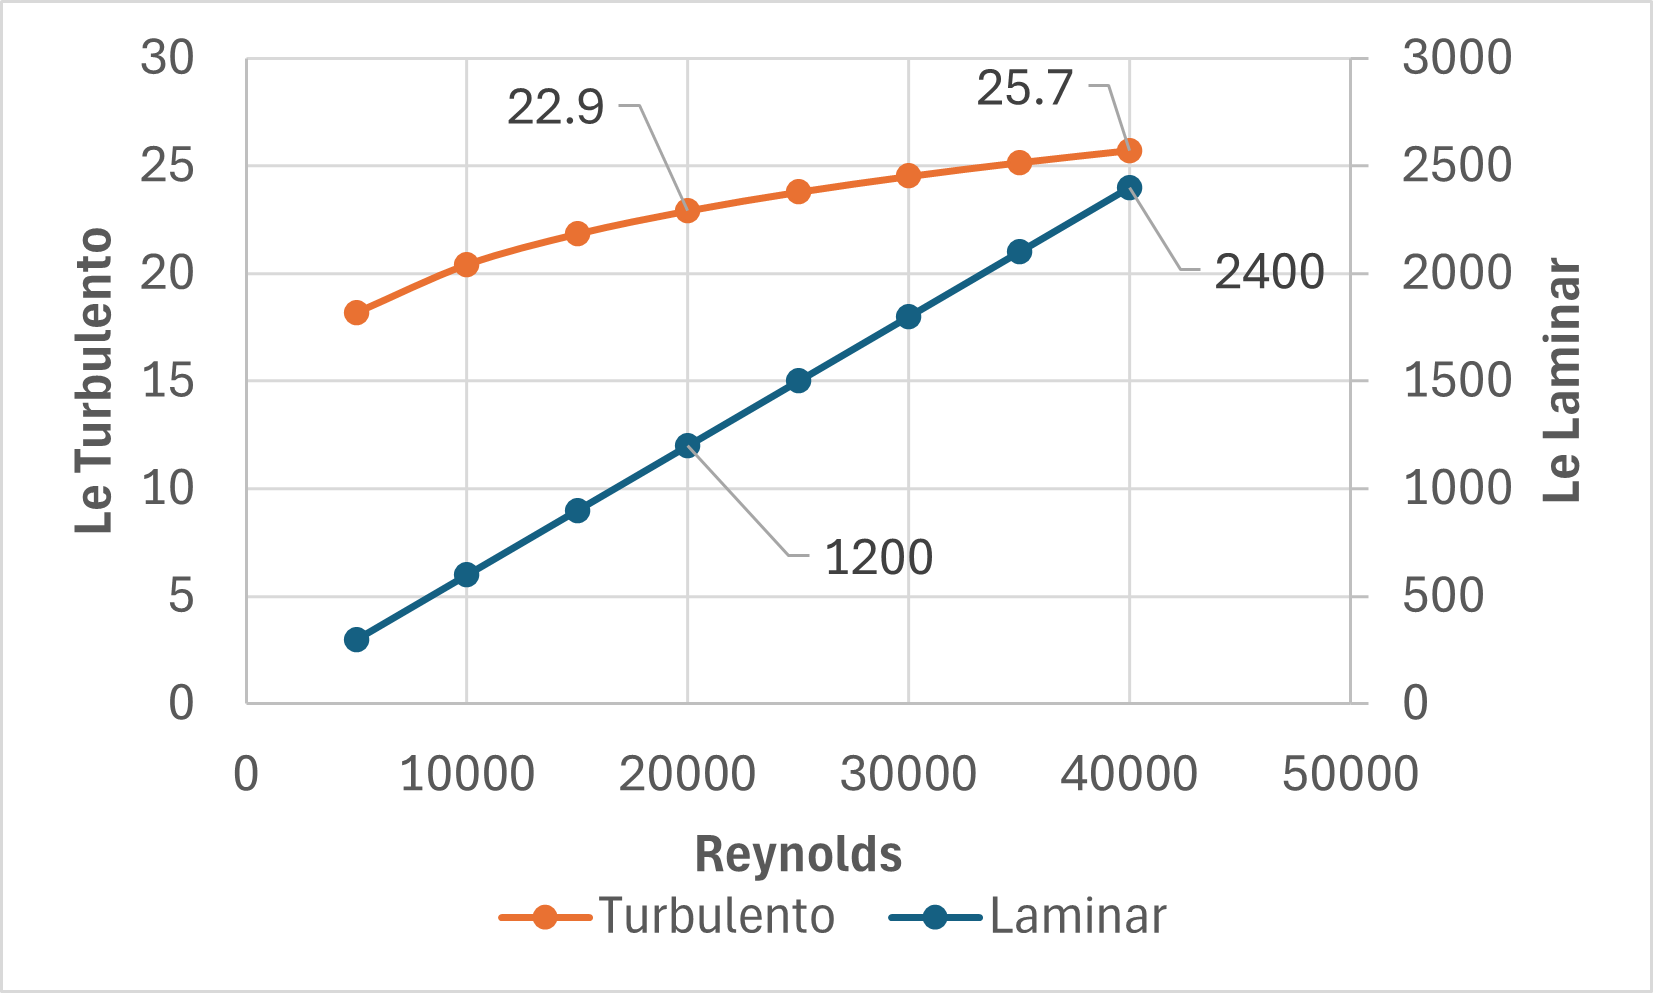
\includegraphics[width=.65\textwidth]{figures/4}
	\caption{Perfil de velocidade para condicões de gradiente nulo, favorãvel e adverso.}
\end{figure}

A curva de perfil sem gradiente de pressão (azul) mostra uma transição suave da parede para a camada externa. Para o gradiente favorável (verde), vemos como ele se achata para altos valores de $\eta$ devido à aceleração do fluxo. Para o gradiente desfavorável, observa-se uma tendência a um déficit menor, com a pendiente aumentando para altos valores de $n$.

Por último, cuando $b \rightarrow\infty$, a condição de separação pode ser encontrada (para o exemplo mostrado $b=50$). O gradiente é casi nulo em regiões perto da parede e para altos valores de $\eta$, a separacao da camada turbulente pode ser deducida.

\begin{figure}[H]
	\centering
	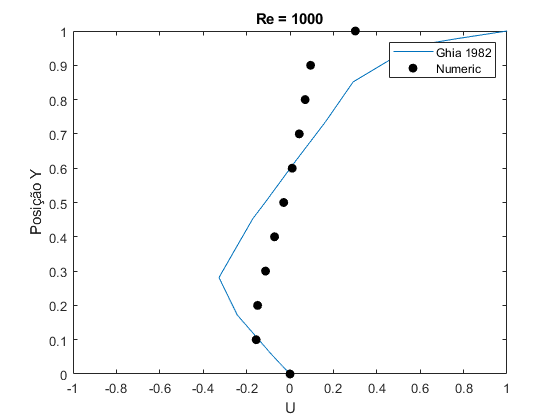
\includegraphics[width=.65\textwidth]{figures/5}
	\caption{Déficit de velocidade para condicões de separacão, favorãvel e adversa.}
\end{figure}

\begin{thebibliography}{999}
	
	
	\bibitem{Deschamps}
	Cesar Deschamps,
	Escalas da turbulencia Cap 3.
	UFSC Florianopolis, SC,
	Notas de aula,
	2025.
	
	\bibitem{abejan}
	Adrian Bejan,
	Convection Heat Transfer.
	Durham, North Carolina,
	3rd Edition,
	2004.
		
	
\end{thebibliography}


\end{document}





